\documentclass{article}

\usepackage{tikz}
\usepackage{pgfkeys}
\usetikzlibrary{mindmap,trees,shapes,calc,fadings}

\tikzset{%
  % Specifications for style of nodes:
    base/.style = {rectangle, rounded corners, draw=black,
                   minimum width=4cm, minimum height=1cm,
                   text centered, font=\sffamily},
    version/.style = {base, fill=green!30},
    virtual/.style = {base, fill=blue!30},
    data/.style = {base, fill=orange!30},
    mark coordinate/.style={inner sep=0pt,outer sep=0pt,minimum size=3pt,
    fill=black,circle}%
}

\newcommand\pgfmathsinandcos[3]{%
  \pgfmathsetmacro#1{sin(#3)}%
  \pgfmathsetmacro#2{cos(#3)}%
}

\newcommand\DrawLatitudeCircle[2][1]{
  \LatitudePlane{\angEl}{#2}
  \tikzset{current plane/.prefix style={scale=#1}}
  \pgfmathsetmacro\sinVis{sin(#2)/cos(#2)*sin(\angEl)/cos(\angEl)}
  % angle of "visibility"
  \pgfmathsetmacro\angVis{asin(min(1,max(\sinVis,-1)))}
  \draw[current plane] (\angVis:1) arc (\angVis:-\angVis-180:1);
  \draw[current plane,dashed] (180-\angVis:1) arc (180-\angVis:\angVis:1);
}

\newcommand\LatitudePlane[3][current plane]{%
  \pgfmathsinandcos\sinEl\cosEl{#2} % elevation
  \pgfmathsinandcos\sint\cost{#3} % latitude
  \pgfmathsetmacro\yshift{\cosEl*\sint}
  \tikzset{#1/.style={cm={\cost,0,0,\cost*\sinEl,(0,\yshift)}}} %
}

\begin{document}

% Sketch to introduce the notation for equations
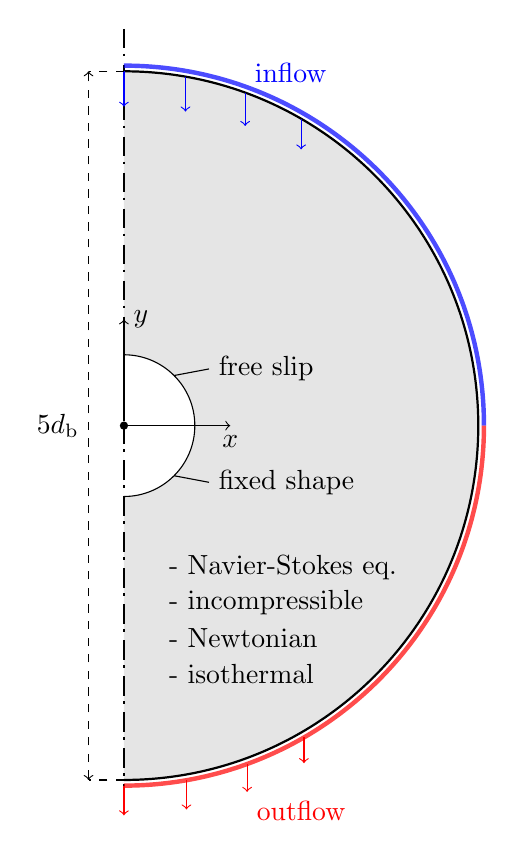
\begin{tikzpicture}[scale=0.9]
\def\R{5.0}
\def\Rv{4.5}
\def\Rvo{5.5}
\def\Rc{5.08}
\def\Rb{1}
\def\Rbi{3}
\def\arcI{90}
\def\arcE{-90}
\def\arcBI{90}
\def\arcBE{30}
\def\arcBIi{15}
\def\arcBEe{0}
\def\Rbii{0.05}
\def\arcBIii{0}
\def\arcBEee{-180}

\coordinate (A) at (0,5);
\coordinate (B) at (0,-5);
\coordinate (Aa) at (0,5.6);
\coordinate (Bb) at (0,-5.5);

\coordinate (B) at (0,0); %start bubble
\coordinate (C) at (0,1.0);
\coordinate (D) at (0.707,0.707);
\coordinate (E) at (0.707,-0.707);
\coordinate (F) at (0.72,-0.2);
\coordinate (G) at (0,-0.6); %end bubble

\filldraw[fill=black,opacity=0.1] (A) arc (\arcI:\arcE:\R);
\filldraw[fill=white,opacity=1.0] (C) arc (\arcI:\arcE:1.0);
%\filldraw[fill=white] (E) to [bend right=30] (F)to [bend right=10] (G) -- (B) to [bend left=23] (C) to [bend left=35] (D) to [bend left=70] (E);

\coordinate[mark coordinate] (O) at (0,0);

\draw [thick] (A) arc (\arcI:\arcE:\R);
\draw[thick,dash pattern={on 7pt off 2pt on 1pt off 3pt}] (Aa) -- (Bb);

\draw[draw,ultra thick,blue,opacity=0.7] (0,\Rc) arc (90:0:\Rc);
\draw[->,blue] ({\R * cos(90)}, {\R * sin(90)}) -- ({\R * cos(90)}, {\Rv * sin(90)});%alpha 80
\draw[->,blue] ({\R * cos(80)}, {\R * sin(80)}) -- ({\R * cos(80)}, {\Rv * sin(80)});%alpha 80
\draw[->,blue] ({\R * cos(70)}, {\R * sin(70)}) -- ({\R * cos(70)}, {\Rv * sin(70)});%alpha 70
\draw[->,blue] ({\R * cos(60)}, {\R * sin(60)}) -- ({\R * cos(60)}, {\Rv * sin(60)});%alpha 60
\draw ({\R * cos(70)}, {\R * sin(70)}) node[above right]{\textcolor{blue}{inflow}};

\draw[draw,ultra thick,red,opacity=0.7] (5.08,0) arc (0:-90:5.08cm);
\draw[->,red] ({\Rc * cos(90)}, {-\Rc * sin(90)}) -- ({\Rc * cos(90)}, {-\Rvo * sin(90)});%alpha 80
\draw[->,red] ({\Rc * cos(80)}, {-\Rc * sin(80)}) -- ({\Rc * cos(80)}, {-\Rvo * sin(80)});%alpha 80
\draw[->,red] ({\Rc * cos(70)}, {-\Rc * sin(70)}) -- ({\Rc * cos(70)}, {-\Rvo * sin(70)});%alpha 70
\draw[->,red] ({\Rc * cos(60)}, {-\Rc * sin(60)}) -- ({\Rc * cos(60)}, {-\Rvo * sin(60)});%alpha 60
\draw ({\Rc * cos(70)}, {-\Rvo * sin(70)}) node[below right]{\textcolor{red}{outflow}};

\coordinate (X) at (1.5,0);
\coordinate (Y) at (0,1.5);
\draw[->] (O) -- (X);
\draw (X) node[below]{$x$};
\draw[->] (O) -- (Y);
\draw (Y) node[right]{$y$};

\coordinate (IO) at ({\R * cos(65)}, {\R * sin(65)});
\coordinate (Ci) at (1.2,0.8);
\draw[color=black] (D) -- (Ci);
\draw[color=black] (Ci) node[right]{free slip};
%\draw[color=black] (Ci) node[below right]{};

\coordinate (PO) at (0.7,-0.2);
\coordinate (POi) at (1.2,-0.8);
\draw[color=black] (E) -- (POi);
\draw[color=black] (POi) node[right]{fixed shape};

\coordinate (E1) at (0.5, -2.0);
\draw (E1) node[right]{- Navier-Stokes eq.};
\coordinate (E2) at (0.5, -2.5);
\draw (E2) node[right]{- incompressible};
\coordinate (E3) at (0.5, -3.0);
\draw (E3) node[right]{- Newtonian};
\coordinate (E4) at (0.5, -3.5);
\draw (E4) node[right]{- isothermal};

%\draw[thick][color=black] (B) to [bend left=23] (C);
%\draw[thick][color=black] (C) to [bend left=35] (D);
%\draw[thick][color=black] (D) to [bend left=70] (E);
%\draw[thick][color=black] (E) to [bend right=30] (F);
%\draw[thick][color=black] (F) to [bend right=10] (G);

\draw[dashed] (0,5) -- (-0.5,5);
\draw[dashed] (0,-5) -- (-0.5,-5);
\draw[<->,dashed] (-0.5,-5) -- (-0.5,5);
\draw (-0.5,0) node[left]{$5 d_{\mathrm{b}}$};
    
\end{tikzpicture}

\end{document}